\documentclass[12pt]{article}

% packages

%\usepackage{times} % alt: cmbright
\usepackage[top=1in, bottom=1in, left=1in, right=1in]{geometry}
\usepackage{natbib}
\usepackage{amsmath}
\usepackage{amssymb}
\usepackage{latexsym}
\usepackage{sectsty}
\usepackage{amsfonts}
\usepackage{epsfig}
\usepackage{url}
\usepackage{microtype}
\usepackage{fixmath}
\usepackage{hyperref}
\usepackage{amsthm}
\usepackage{subfigure}
\usepackage{float}
\usepackage{hyperref}

\newtheorem{lem}{Lemma}
\newtheorem{defn}{Assumption}
\newtheorem{propty}{Property}
\newtheorem{thm}{Theorem}

% references

\newcommand{\mysec}[1]{Section~\ref{sec:#1}}
\newcommand{\myapp}[1]{Appendix~\ref{app:#1}}
\newcommand{\myeq}[1]{Equation~\ref{eq:#1}}
\newcommand{\myeqp}[1]{Eq.~\ref{eq:#1}}
\newcommand{\mychap}[1]{Chapter~\ref{chap:#1}}
\newcommand{\myfig}[1]{Figure~\ref{fig:#1}}

% math conveniences

\newcommand{\g}{\,\vert\,}
\newcommand{\E}{\textrm{E}}
\newcommand{\vct}[1]{\textbf{#1}}
\newcommand{\realline}{\mathbb{R}}
\newcommand{\indpt}{\protect\mathpalette{\protect\independenT}{\perp}}
\def\independenT#1#2{\mathrel{\rlap{$#1#2$}\mkern2mu{#1#2}}}
\newcommand{\h}[1]{\textrm{H}\left( #1 \right)}
\newcommand{\half}{\frac{1}{2}}
\newcommand{\new}{\textrm{new}}

\newcommand{\mult}{\textrm{Mult}}
\newcommand{\dir}{\textrm{Dir}}
\newcommand{\discrete}{\textrm{Discrete}}
\newcommand{\Bern}{\textrm{Bern}}
\newcommand{\DP}{\textrm{DP}}
\newcommand{\GP}{\textrm{GP}}
\newcommand{\Bet}{\textrm{Beta}}

% paragraph spacing

\setlength{\parindent}{0pt}
\setlength{\parskip}{2ex plus 0.5ex minus 0.2ex}

\allsectionsfont{\sffamily\mdseries}
\paragraphfont{\sffamily\bfseries}

\usepackage{algorithm}
\usepackage{algorithmic}
\renewcommand{\algorithmicrequire}{\textbf{Input:}}
\renewcommand{\algorithmicensure}{\textbf{Output:}}


\begin{document}

\title{\textsf{Informative Path Planning for a Wingman Robot in a Collaborative Search Task}}
%\author{\textsf{Daqing Yi} \and \textsf{Michael A. Goodrich}}
\date{\textsf{Brigham Young University}}

\maketitle

\section{Introduction}

\subsection{Cordon and Search}

Cordoning off an area and searching for insurgent objects has been proved to be an effective tactic in complex environments. It is one of the most frequently used tasks in the Global War on Terror. The cordon task serves as a security element of the entire team, which prevents withdrawal from or reinforcement of a position so that the search could be executed effectively and fluently. Once a cordon is established, the search task focuses
on walking through the search space to find target personnel or material.

Both the cordon task and the search task involve information gathering in the form of a multi-agent team. Members of the team often work under tight time constraint or are exposed to risk. Consequently, it is natural to consider including robots in a cordon and search team. The advantages of involving robots in a cordon and search team potentially include: \\
(1) Assigning some tasks to a robot might reduce potential danger to humans. \\
(2) Robots can deliver constant and stable performance without fatigue. \\
(3) From the versatility of sensors equipped, robots can extend the perception capability of the entire team.

\subsection{Robot Wingman}

Both the cordon and search phase include an element of discovering the environment. Moving into position for a cordon is often dangerous, and requires an ongoing evaluation of information in the world. To support both explicit search from the search phase and the implicit search associated with the cordon phase, \cite{goodrich2013toward} introduce a robot wingman. 

The robot wingman defines a type of human-robot relationship in a team, which is to have a robot that accompanies a human when the human navigates through
some space. With versatile sensors, the robot wingman might detect threats or opportunities that may be relevant to the human but likely not seen by the human. The robot wingman in a team enlarges the geographical region of observation, and expands the perception of the team as an entity.

\section{Related Works}

The existence of robot motion brings a path planning process. Instead of blind random walking, the path planning usually targets at optimizing specific objectives, which helps the motion efficiency [\cite{goodrich2013toward}]. In a search problem, the objective function is usually defined as information maximization. The motion constraint usually converts a graph to a larger scale spanning tree, which increases the complexity. \cite{levine2010information} proposes information-rich RRT to generate a path for target tracking. Using a receding horizon planning idea, \cite{JonesSchwagerBeltaICRA13scLTLInfo} uses an information gathering path planning algorithm with a temporal logic constraint.

Considering the observation of an agent might not only cover the visit point but a neighboring area, the problem can be defined as a "Maximum Coverage Problem". The reward collected at each step is not constant but depends on the path has been through, which also forms a submodular maximization problem. \cite{singh2009efficient} proposes an efficient search algorithm in simple greedy framework with problem decomposition. In non-teleport motion, \cite{chekuri2005recursive} imports recursive greedy by converting to knapsack constraint. Similarly, in a brand and bound way, \cite{binney2012branch} applies greedy search to informative path planning. These cannot work in Robot wingman problem, the motion of which constrains in a strict pace with the human through time so that we are not able to convert time to budget in an optimization problem.

In this paper, we will model the robot wingman problem and propose an algorithm to solve the problem in considering both performance and efficiency. In the end, we will use simulation to support the algorithm proposed and analyze the impact from several factors. 

To evaluate the performance of an algorithm on path planning in robot wingman framework, we focus on four principles.
\begin{itemize}
\item obeys consistency principle;
\item guaranteed bounds on how close the solution is to suboptimal;
\item is computationally tractable;
\item is useful for real robots in the wingman problem.
\end{itemize}

\section{Problem Statement}

\begin{figure}[htbp]
\centering
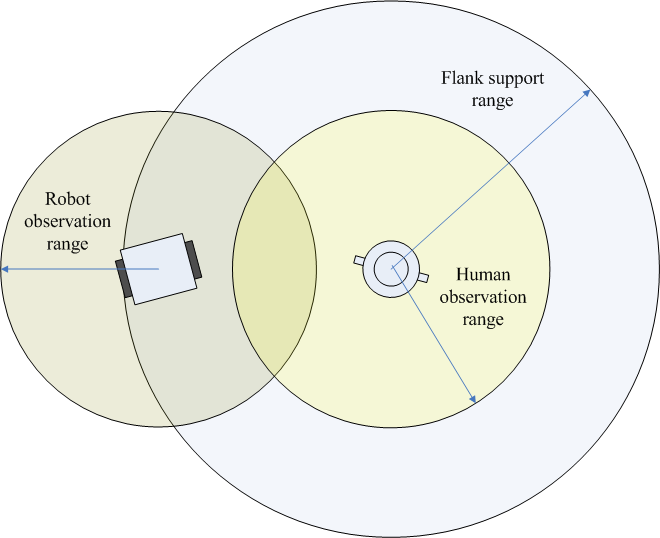
\includegraphics[width=0.4\textwidth]{./images/Wingman}
\caption{A Robot Wingman Framework.}
\label{fig:Wingman}
\end{figure}

We define a flank support range to present the constraint on wingman motion, which determines the area that a robot wingman is expected to stay in when a human is moving. The search space is discretized into cells, which forms the topology defining the connectivities between accessible positions, as in Fig.\ref{fig:LayerStructure}. In a search problem on a discrete map, we denote $ P(S_{i}) $ as the probability of the search target at position $ i $, and $ H(S_{i}) $ as its corresponding entropy. The motion of an agent in the search space turns to visiting the cells in the discrete map or the vertices in the topology. Like in Fig.\ref{fig:Wingman}, we assume both human and robot can observe a circular area around, which is defined by observation range. In a discrete map, this observation model means an agent can observe not only the visited cell but neighboring cells in a range. Here a neighbor function $ n(\cdot) $ is used to denotes all the neighboring cells of a given node that satisfy some constraints. $ n_{flank}^{human}(\cdot) $ defines the allowable cells for the robot's location given the human's position, $ n^{human}(\cdot) $  and $ n^{robot}(\cdot) $ define the observable cells given a position by human and robot correspondingly. 


\begin{figure}[htbp]
\centering
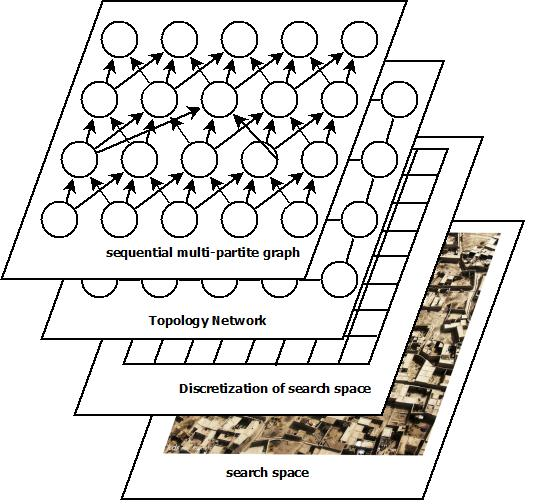
\includegraphics[width=0.4\textwidth]{./images/LayerStructure}
\caption{A Layer Structure of Problem Abstraction from Real World of Search Space to Topological Descripition.}
\label{fig:LayerStructure}
\end{figure}

\subsection{Human Path Dependence}

In a time length of $ T $, let a vector $ Y = [y_{1}, y_{2} \cdots , y_{T}] $ define a path of the human. Similarly, we have a path of the robot as $ X = [x_{1}, x_{2} \cdots, x_{T}] $. For simplification, we have   or $ \textbf{O}^{Y} $ to denote the observations on neighboring cells when a robot is at cell $ x $ or a human is at cell $ y $. In this scenario, the information gain of the robot is defined by conditional mutual information. In equation (\ref{eq:condMutInf}), it means the entropy reduction on the search space $ \textbf{S} $ due to the observation of a robot $ \textbf{O}^{X} $ when the observation of a human $ \textbf{O}^{Y} $ is given.

\begin{equation}
\label{eq:condMutInf}
\begin{aligned}
I(\textbf{S}; \textbf{O}^{X} \mid \textbf{O}^{Y}) & = H(\textbf{S} \mid \textbf{O}^{Y}) - H(\textbf{S} \mid \textbf{O}^{X},\textbf{O}^{Y})\\
& = H(\textbf{O}^{X} \mid \textbf{O}^{Y}) - H(\textbf{O}^{X} \mid \textbf{O}^{Y}, \textbf{S}).
\end{aligned}
\end{equation}

The problem can be defined as:

\begin{equation}
\label{eq:objFunc}
\begin{aligned}
Objective: X^{*} = \underset{X}{\arg\max} [I(\textbf{S}; \textbf{O}^{X} \mid \textbf{O}^{Y})] \\
Constraint: \forall t, x^{t} \in n^{human}_{flank}(y_{t}) \cap n^{robot}_{1}(x^{t-1}) 
\end{aligned}
\end{equation}

\begin{defn}
\label{Assumption1}

The human path is known.

\end{defn}

Assume the human path can be predicted, by which we can known $ \textbf{O}^{Y} $. With $ \textbf{O}^{Y} $ given, the uncertainty estimation of the search space can be updated before path planning of the robot. 

\begin{lem} 
\label{Lemma1}
When the human observation $ \textbf{O}^{Y} $ is known, we have:
\begin{equation}
\label{eq:offHmPathChain}
\begin{aligned}
I(\textbf{S}; \textbf{O}^{X} \mid \textbf{O}^{Y}) & = \sum_{t=1}^{T} H(O_{t}^{X} \mid O_{t-1}^{X} \cdots, O_{1}^{X}, \textbf{S}, \textbf{O}^{Y}) - \sum_{t=1}^{T} H(O_{t}^{X} \mid O_{t-1}^{X} \cdots, O_{1}^{X}, \textbf{O}^{Y})\\
& = \sum_{t=1}^{T} I(O^{X}_{t} ; \textbf{S} \mid O^{X}_{t-1} \cdots O^{X}_{1}, \textbf{O}^{Y})
\end{aligned}
\end{equation}
\end{lem}

This gives the reward collected at each step in a chain rule manner. 

\subsection{Unfold Solution Space of Single Step Through Time}

When assumption \ref{Assumption1} stands, we can see that wingman constraint gives a limited solution space for each step of a time. Unfolding the solution space of single step through planning time, we can have a multi-partite graph. Partite $ t $ contains all of the cells in $ n^{human}_{flank}(y_{t}) $, and the connectivities between two partites are determined by the topology generated from discrete map.

\begin{figure}[htbp]
\centering
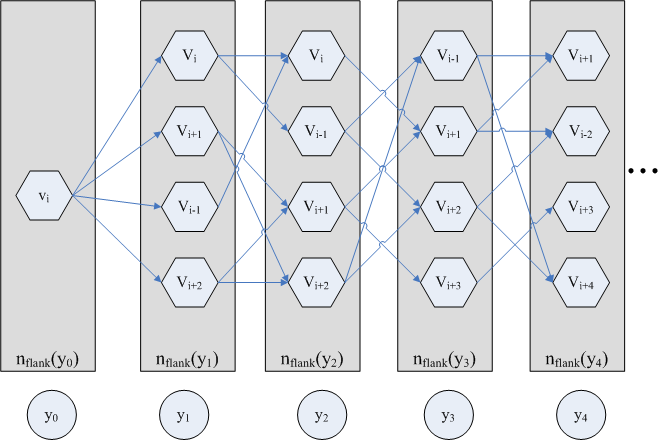
\includegraphics[width=0.4\textwidth]{./images/MultiPartite}
\caption{A multi-partite graph for robot wingman search.}
\label{fig:MultiPartite}
\end{figure}

The path planning under wingman constraint has been converted to path planning on a multi-partite graph. In a search process, it restricts the search direction, moving to next partite at next step. A vertex in a partite which cannot be reached from the previous partite or cannot reach next
partite is not a valid choice in a time step. So a prune process can be used to remove ``meaningless" vertices, which can be achieved through forward
pruning and backward pruning. After pruning, we have a directed multi-partite graph like in Fig.\ref{fig:MultiPartite}, which has the properties:
\begin{enumerate}
\item At step $ 1 $, $ \forall $ vertex $ v \in $ partite $ V_{1} $, $ deg^{+}(v) > 0 $ and $ deg^{-}(v) = 0 $;
\item At step $ T $, $ \forall $ vertex $ v \in $ partite $ V_{T} $, $ deg^{+}(v) = 0 $ and $ deg^{-}(v) > 0 $;
\item At step $ t \in (1, T) $, $ \forall $ vertex $ v \in $ partite $ V_{t} $, $ deg^{+}(v) > 0 $ and $ deg^{-}(v) > 0 $.
\end{enumerate}

The guarantee of connectivities between choices at time $ t $ and time $ t+1 $ asks the problem solving by time sequence.

\subsection{Observation Model}

By Fig.\ref{fig:Wingman}, we know that $ \textbf{O}^{X} $ and $ \textbf{O}^{Y} $ are determined by  $ n^{robot}(\cdot) $ and  $ n^{human}(\cdot) $ respectively. The observation model determines how the uncertainty reduction will be when observing at one position, and each observation will update the uncertainty estimation on the search space. 

When an agent only observes visited position, the problem is like most of the classical optimization problem. Equation (\ref{eq:offHmPathChain}) will become $ I(\textbf{S}; \textbf{O}^{X} \mid \textbf{O}^{Y}) = \sum_{t=1}^{T} I(O^{X}_{t} ; \textbf{S} \mid \textbf{O}^{Y})  $ if we constantly remove choices made from solution space. From a perspective of reward collecting, a current step will not influence the reward in a future step. When an agent extends the observation to a detection range, the problem moves to a ``Maximum Coverage Problem", in which there can be a overlap between two different steps. It means a current step might influence the reward in a future step. The submodularity shows that if $ s_{i} \in  n^{robot}(x_{t}) $ and $ s_{i} \in  n^{robot}(x_{t+k}) $, $ H_{t}(s_{i}) \geq H_{t+k}(s_{i}) $, because the uncertainty estimation at $ s_{i} $ has been updated at step $ t $. The way of defining observation model makes reward at a position depends on the choices already have been made. It forms a ``Path-Dependent Optimization Problem".

Moreover, when an agent works in field, which usually has complex environment description, there are more factors determining the detection likelihood of an observation model, as in Fig.\ref{fig:obsFactors}. Fig.\ref{fig:detectRange} shows how the detection range can be blocked by obstacles, while Fig.\ref{fig:visibilityGraph} and Fig.\ref{fig:viewshed} gives how the visibility graph and viewshed can influence the detection likelihood in different positions. 

\begin{figure}
\centering
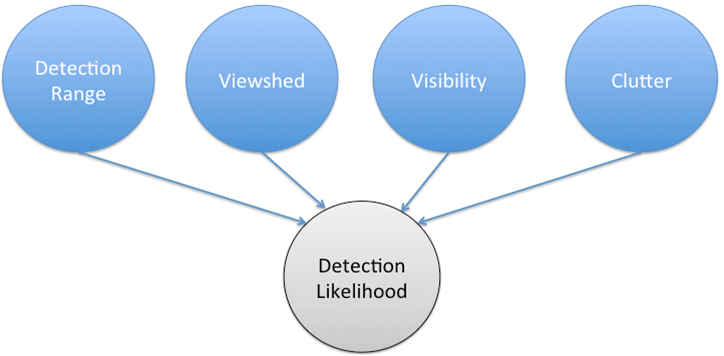
\includegraphics[width=0.7\linewidth]{./images/obsFactors}
\caption{Factors that determine the detection likelihood of an observation model.}
\label{fig:obsFactors}
\end{figure}

\begin{figure} 
  \centering 
  \subfigure[Detection Range]{ 
    \label{fig:detectRange} %% label for first subfigure 
    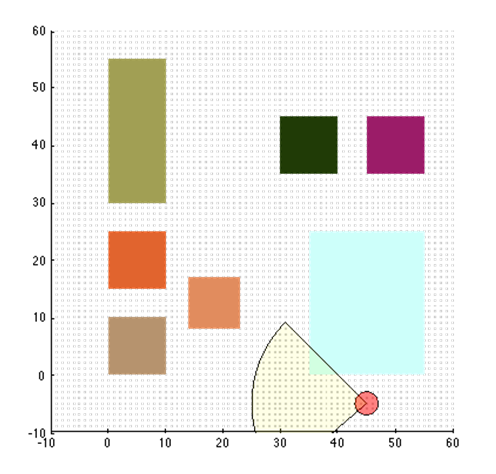
\includegraphics[width=0.3\textwidth]{./images/detectRng.png}} 
  %\hspace{1in} 
  \subfigure[Visibility Graph]{ 
    \label{fig:visibilityGraph} %% label for second subfigure 
    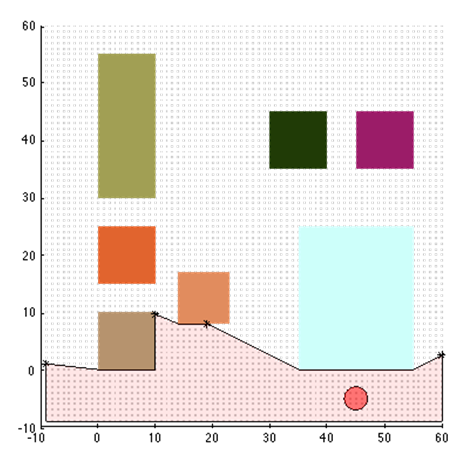
\includegraphics[width=0.3\textwidth]{./images/visbilityGraph.png}} 
  \subfigure[Viewshed]{ 
    \label{fig:viewshed} %% label for second subfigure 
    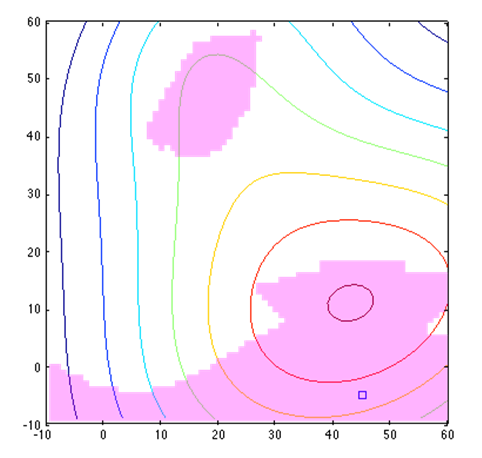
\includegraphics[width=0.3\textwidth]{./images/viewshed.png}}     
  \caption{How the observation model is influenced.}
  \label{fig:factorsOnObs} %% label for entire figure 
\end{figure}

\section{Path-Dependent Optimization}

In a path-dependent optimization problem, the reward can be collected at one step might depend on the previous steps, which is path-dependent. Expressing in a generic form, we use $ f(\cdot) $ to denote any function which can be used to quantify the reward collected at one step. In our case, $ f(\cdot) $ considers overlap reward function, motion constraint and observation model. So we can rewrite Equation (\ref{eq:objFunc}) as 

\begin{equation}
\label{eq:gnr_obj}
Objective: X^{*} = \underset{X}{\arg\max} f(X)
\end{equation}

From Lemma \ref{Lemma1}, we can write
\begin{equation}
\label{eq:gnr_f_chain}
f(x_{1}, x_{2}, \cdots x_{T}) = f(x_{1}) + f(x_{2} \mid x_{1}) + \cdots f(x_{T} \mid x_{T-1}, \cdots x_{1}).
\end{equation}

By Equation (\ref{eq:gnr_obj}), we have

\begin{equation}
\label{eq:max_1}
\begin{aligned}
& \max_{X} f(X) \\
& = \max_{X_{1}, X_{2} \cdots X_{T}} f(x_{1}, x_{2}, \cdots x_{T}) \\
& = \max_{X_{1}, X_{2} \cdots X_{T}} \left[ f(x_{1}) + f(x_{2} \mid x_{1}) + \cdots f(x_{T} \mid x_{T-1}, \cdots x_{1}) \right] \\
& = \max_{X_{1}} \left[ f(x_{1}) + \max_{X_{2}} \left[ f(x_{2} \mid x_{1}) + \cdots + \max_{X_{T}} f(x_{T} \mid x_{T-1}, \cdots x_{1}) \right] \right].
\end{aligned}
\end{equation}

Let 
\begin{equation}
\label{eq:max_2}
\hat{x}_{t} = \arg \max_{X_{t}} \left[ f(x_{t} \mid x_{t-1}, \cdots x_{1})
+ \max_{X_{t+1}, \cdots X_{T}} f(x_{T}, \cdots x_{t+1} \mid x_{t}, \cdots x_{1})
\right],
\end{equation}

we can have the problem decomposed into solving optimal problem at each step,

\begin{equation}
\label{eq:max_3}
\begin{aligned}
x_{1}^{*} & = \arg \max_{X_{1}} \left[ f(x_{1}) + \max_{X_{t+1}, \cdots X_{T}} f(x_{T}, \cdots x_{t+1} \mid x_{t}, \cdots x_{1})  \right]; \\
x_{2}^{*} & = \arg \max_{X_{2}} \left[ f(x_{2} \mid x_{1}^{*}) + \max_{X_{3}, \cdots X_{T}} f(x_{T}, \cdots x_{3} \mid x_{2}, \cdots x_{1}^{*})  \right]; \\
& \cdots \\
x_{t}^{*} & = \arg \max_{X_{t}} \left[ f(x_{t} \mid x_{t-1}^{*}, \cdots x_{1}^{*}) + \max_{X_{t+1}, \cdots X_{T}} f(x_{T}, \cdots x_{t+1} \mid x_{t},  x_{t-1}^{*}, \cdots x_{1}^{*}) \right]; \\
& \cdots \\
x_{T}^{*} & = \arg \max_{X_{T}} \left[ f(x_{T} \mid x_{T-1}^{*}, x_{T-2}^{*}, \cdots x_{1}^{*})\right].
\end{aligned}
\end{equation}

We can see that at time $ t $, 
$ f(x_{t} \mid x_{t-1}^{*}, \cdots x_{1}^{*}) $ is the instant reward of choosing a $ x_{t} $. While $ \max_{X_{t+1}, \cdots X_{T}} f(x_{T}, \cdots x_{t+1} \mid x_{t},  x_{t-1}^{*}, \cdots x_{1}^{*}) $ denotes the future reward of choosing a $ x_{t} $ assuming that optimal choices will be made in the future steps given choices from time $ 1 $ to $ t $.

It is clear that at time $ t $, $ f(x_{t} \mid x_{t-1}^{*}, \cdots x_{1}^{*}) $ can be calculated directly with $ x_{1} \cdots x_{t} $ given. While $ \max_{X_{t+1}, \cdots X_{T}} f(x_{T}, \cdots x_{t+1} \mid x_{t},  x_{t-1}^{*}, \cdots x_{1}^{*}) $ is something exists but hard to calculate, especially it depends on that the choices from step $ 1 $ to step $ t-1 $ are optimal. For short, it will be written as $ h(x_{t},  x_{t-1}, \cdots x_{1}) = \max_{X_{t+1}, \cdots X_{T}} f(x_{T}, \cdots x_{t+1} \mid x_{t},  x_{t-1}, \cdots x_{1}) $ in the latter section. Equation \ref{eq:max_3} tells that if each step can always know how the future reward is and sequentially make the best choice, an optimal solution can be found. Here the problem turns to how to estimate the future reward so that an optimal solution can be approximated.

\section{A Tree-Expanding Search with Recursive Backtracking}

Given a start node, any search problem on a graph implicitly derives an expanding tree, the root of which is the start node. In a multi-partite graph of $ T $ levels, an expanding tree also has depth of $ T $. In this paper, ``terminal node" is named for any node at the depth of planning length $ T $. As a node in $ t $ level of expanding tree can be mapped to a path $ x_{1}, x_{2} \cdots x_{t} $, a terminal node implies a complete path of length $ T $. 

\begin{propty}
\label{prop:path}
Each expanding node $ v $ of $ x_{t} $ implies a path $ path(v) = \{ x_{1}, x_{2} \cdots x_{t} \}  $.
\begin{proof}
From the root of an expanding tree $ v_{root} $, there exist one and only path to any other expanding node $ v $. 
\end{proof}
\end{propty}

Brute Force Search will have to expand all possible terminal nodes so that it can find the optimal. A greedy search has the advantage of efficiency, which expands only a branch of an expanding tree but can often be misled by local optimal. Submodularity provides performance guarantee, but in the constraint of continuous motion, the performance can be extremely low. Importing heuristic usually provides more future information, which helps the node choosing in search.

Considering the search direction consistency in this directed multi-partite graph structure, we import a backtracking process to back propagate information to a time step in decision, which is used to estimate maximum future reward given previous choices, approximating $ h(x_{t},  x_{t-1}, \cdots x_{1}) $. The algorithms are given in Algorithm \ref{alg:Backtrack}.

\subsection{Backtracking Algorithm}

\begin{algorithm}
\caption{Backtracking}
\label{alg:Backtrack}
\begin{algorithmic}
\REQUIRE
Expanding Node $ v $, Multi-partite graph $ G $;
\ENSURE $ \hat{h}(path(v)) $ ;\\
\STATE $ T = G.length $;
\STATE $ path(v) = \{ x_{1}, x_{2} \cdots x_{t'} \} $;
\FOR{ $ t=T:1:t'+1 $ }
\FOR{ $ x_{t} \in G[t] $}
\IF {$ t == T $}
\STATE $ \hat{f}(x_{T} \mid path(v) ) = f(x_{t} \mid path(v)) $
\ELSE
\STATE $ \hat{f}(x_{T} \cdots x_{t} \mid path(v) ) = \max_{x_{t+1} \in n^{robot}_{1}(x_{t})} \hat{f}(x_{T} \cdots x_{t+1} \mid path(v) ) +  f(x_{t} \mid path(v)) $
\ENDIF
\ENDFOR
\ENDFOR
\STATE  $ \hat{h}(path(v)) = \max_{x \in G[t+1]} \hat{h}(x, x_{T} \cdots x_{t+1} \mid path(v) ) $
\RETURN $ \hat{h}(path(v))  $
\end{algorithmic}
\end{algorithm}
%Backtrack process provides all the possible future rewards of next step $ \hat{R}^{max}_{future}(x_{path(v).length+1} \mid path(v) ) $. Selecting the maximum, we can used this as the estimation on future reward of node $ v $, $ est_{max}(R^{max}_{future}(v)) $.

$ f(x_{t} \mid path(v)) $ is the reward can be collected at $ x_{t} $ considering only $ path(v) $. From the submodularity of a sequential coverage problem, we know 
\begin{equation}
\label{eq:submod1}
\begin{aligned}
f(x_{t} \mid path(v)) \geq f(x_{t} \mid \hat{x}_{t-1} \cdots \hat{x}_{t'+1}, path(v) ),
t' = path(v).length,
\end{aligned}
\end{equation}

the actual reward can be collected at $ x_{t} $ should be less or equal to $ f(x_{t} \mid path(v)) $. $ \hat{h}(path(v)) $ gives the estimated maximum future reward after walking $ path(v) $. $ \hat{f}(x_{T} \cdots x_{t'} \mid path(v) ) $ is defined as the estimated total reward from $ x_{T} \cdots x_{t'} $ after walking $ path(v) $.

%$ f(x_{t} \mid \hat{x}^{*}_{t-1}, \cdots \hat{x}^{*}_{1}) $ means instant reward of choosing $ x_{t} $ with path $ \hat{x}^{*}_{t-1}, \cdots \hat{x}^{*}_{1} $ given. $ \tilde{f}(\tilde{x}^{*}_{T}, \cdots \tilde{x}^{*}_{t+1} \mid x_{t}, \hat{x}^{*}_{t-1}, \cdots \hat{x}^{*}_{1} ) $ is the estimated maximum future reward of choosing $ x_{t} $ with path $ \hat{x}^{*}_{t-1}, \cdots \hat{x}^{*}_{1} $ given. $ \hat{F}^{*}(x_{t} \mid \hat{x}^{*}_{t-1}, \cdots \hat{x}^{*}_{1}) $ is the estimated reward of choosing $ x_{t} $ with path $ \hat{x}^{*}_{t-1}, \cdots \hat{x}^{*}_{1} $ given, including instant reward and estimated future reward.

\begin{propty}
\label{prop:underestimate}
``Backtracking" in Algorithm \ref{alg:Backtrack} will never underestimate the future reward.
\begin{proof}

Let $ g(x_{t} \mid path(v)) $ be maximum future reward starting from $ x_{t} $ with $ path(v) $ given. Let $ t' = path(v).length $. We know that $ x_{t'+1} \in G[t'+1], g(x_{t'+1} \mid path(v)) $ shows maximum future rewards of all the nodes at level $ t'+1 $. $ \max_{x_{t'+1} \in n^{robot}_{1}(v)} g(x_{t'+1} \mid path(v)) $ equals to the maximum future reward from $ path(v) $. Also we can have:

\begin{equation}
\begin{aligned}
g(x_{t} \mid path(v)) = \max_{x_{t+1} \in n^{robot}_{1}(x_{t})} g(x_{t+1} \mid path(v)) + f(x_{t} \mid \tilde{x}_{t+1}, \cdots \tilde{x}_{T}, path(v)),
\end{aligned}
\end{equation}

in which $ \tilde{x}_{t+1}, \cdots \tilde{x}_{T} $ are the implicit maximum node sequence makes $ g{x_{t} \mid path(v)} $ maximum future reward. 

Let $ \hat{g}(x_{t} \mid path(v)) $ be estimated maximum future reward starting from $ x_{t} $ with $ path(v) $ given, which is obtained by backtracking in Algorithm \ref{alg:Backtrack}. Similarly, we have:

\begin{equation}
\begin{aligned}
\hat{g}(x_{t} \mid path(v)) = \max_{x_{t+1} \in n^{robot}_{1}(x_{t})} \hat{g}(x_{t+1} \mid path(v)) + f(x_{t} \mid path(v)).
\end{aligned}
\end{equation}

At time $ T $, we have
\begin{equation}
\begin{aligned}
g(x_{T} \mid path(v)) = f(x_{T} \mid path(v))
\end{aligned}
\end{equation}
and
\begin{equation}
\begin{aligned}
\hat{g}(x_{T} \mid path(v)) = f(x_{T} \mid path(v)),
\end{aligned}
\end{equation}

so 
\begin{equation}
\label{eq:inductionInit}
\begin{aligned}
\hat{g}(x_{T} \mid path(v)) = g(x_{T} \mid path(v)).
\end{aligned}
\end{equation},

At any time $ t $, if 
\begin{equation}
\label{eq:inductionAssumption}
\begin{aligned}
\forall x_{t+1}, \hat{g}(x_{t+1} \mid path(v)) \geq g(x_{t+1} \mid path(v)),
\end{aligned}
\end{equation}
we have
\begin{equation}
\begin{aligned}
& \hat{g}(x_{t} \mid path(v)) - g(x_{t} \mid path(v)) \\
& = ( \max_{x_{t+1} \in n^{robot}_{1}(x_{t})} \hat{g}(x_{t+1} \mid path(v)) - \max_{x_{t+1} \in n^{robot}_{1}(x_{t})} \hat{g}(x_{t+1} \mid path(v)) ) \\
& + ( f(x_{t} \mid path(v)) - f(x_{t} \mid \tilde{x}_{t+1}, \cdots \tilde{x}_{T}, path(v)) ).
\end{aligned}
\end{equation}

By submodularity, 
\begin{equation}
\label{eq:inductionGEQ1}
f(x_{t} \mid path(v)) - f(x_{t} \mid \tilde{x}_{t+1}, \cdots \tilde{x}_{T}, path(v)) \geq 0 .
\end{equation}
 

Assume $ x^{a}_{t+1} = \arg \max_{x_{t+1} \in n^{robot}_{1}(x_{t})} \hat{g}(x_{t+1} \mid path(v))  $ and $ x^{b}_{t+1} = \arg \max_{x_{t+1} \in n^{robot}_{1}(x_{t})} g(x_{t+1} \mid path(v)) $, we have
\begin{equation}
\begin{aligned}
\hat{g}(x^{a}_{t+1} \mid path(v)) \geq \hat{g}(x^{b}_{t+1} \mid path(v))
\end{aligned}
\end{equation}
and
\begin{equation}
\begin{aligned}
\hat{g}(x^{b}_{t+1} \mid path(v)) \geq g(x^{b}_{t+1} \mid path(v))
\end{aligned}
\end{equation}
by Equation (\ref{eq:inductionAssumption}).

So 
\begin{equation}
 \hat{g} \( x^{a}_{t+1} \mid path(v) \) \geq  g \( x^{b}_{t+1} \mid path(v) \)
\end{equation} 
 , which means
\begin{equation}
\label{eq:inductionGEQ2}
\begin{aligned}
\max_{x_{t+1} \in n^{robot}_{1}(x_{t})} \hat{g}(x_{t+1} \mid path(v)) - \max_{x_{t+1} \in n^{robot}_{1}(x_{t})} \hat{g}(x_{t+1} \mid path(v)) \geq 0.
\end{aligned}
\end{equation}

With Equation (\ref{eq:inductionGEQ1}) and (\ref{eq:inductionGEQ2}), we have
\begin{equation}
\label{eq:induction}
\forall x_{t+1}, \hat{g}(x_{t+1} \mid path(v)) \geq g(x_{t+1} \mid path(v)) \Rightarrow  \forall x_{t}, \hat{g}(x_{t} \mid path(v)) \geq g(x_{t} \mid path(v))
\end{equation}

With Equation (\ref{eq:inductionInit}) and Equation (\ref{eq:induction}), applying induction we can have
\begin{equation}
\label{eq:inductionResult}
\forall x_{t'+1}, \hat{g}(x_{t'+1} \mid path(v)) \geq g(x_{t'+1} \mid path(v)).
\end{equation}

By Equation(\ref{eq:inductionResult}), we have
\begin{equation}
\begin{aligned}
\max_{x_{t'+1} \in n^{robot}_{1}(v)} \hat{g}(x_{t'+1} \mid path(v)) \geq \max_{x_{t'+1} \in n^{robot}_{1}(v)} g(x_{t'+1} \mid path(v)) \\
t' = path(v).length
\end{aligned}
\end{equation}

So we arrive to the conclusion that ``Backtracking" in Algorithm \ref{alg:Backtrack} will never underestimate the future reward.


%Consider from a ``Sequential Coverage Problem", as we have Equation(\ref{eq:submod1}), 
%\begin{equation}
%\begin{aligned}
%& \sum\limits_{t'+1}^{T} f(x_{t} \mid \hat{x}_{t-1} \cdots \hat{x}_{t'+1}, path(v) )
%\leq & \sum\limits_{t'+1}^{T} f(x_{t} \mid path(v)), t' = path(v).length
%\end{aligned}
%\end{equation}

%Consider from a set operation, the total future reward should be calculated from set union of observed positions. However, ``Backtracking" runs in a summation way to accumulate future reward. So we have
%$ \sum\limits_{t}^{T} Obs(x_{t}) \geq \bigcap\limits_{t}^{T} Obs(x_{t}) $.

\end{proof}
\end{propty}

%With the rewards of all choices estimated from Algorithm \ref{alg:Backtrack}, we propose a ``Recursive Backtracking" to generate paths. In Algorithm \ref{alg:RecursiveBacktrack}, a recursive process is imported to update the uncertainty estimation on search space after one step choice has been made, which corrects $ f(x_{t} \mid \hat{x}^{*}_{t-1}, \cdots \hat{x}^{*}_{1}) $ in ``Backtracking". 

%The estimated does not always match the real values, but in most of the cases it shows the correct tendency in choice making. Also, we can see that when the observation range shrinks to only visited position, which means there is no overlap, ``recursive backtracking algorithm" always guarantees to be optimal. Meanwhile, when a multi-partite graph is in a complete structure, ``recursive backtracking algorithm" equals to a simple greedy.


\subsection{Tree Expanding Search}

At each step of finding a solution, recursively call ``Backtracking" will have the estimation better approximating to true value, since the estimation model of $ G $ is updated at each step of a path. Integrating ``Recursive Backtracking" into "Node Expanding" process, we have Algorithm \ref{alg:RecursiveBacktrack}. 

\begin{algorithm}
\caption{Node Expanding with Recursive Backtracking}
\label{alg:RecursiveBacktrack}
\begin{algorithmic}
\REQUIRE 
Expanding Node $ v $, Multi-partite graph $ G $;
\ENSURE $ solution $ as the path planned;
\STATE $ solution = path(v) $ 
\STATE $ T = G.length $
\STATE $ t' = path(v).length $
\FOR{ $ t=t':1:T-1 $ }
\STATE  Expand node $ v $ to get $ child(v) $;
\FOR{ $ v' $ in $ child(v) $ }
\STATE  calculate $ f(path(v')) $;
\STATE  ``Backtracking" to get $ \hat{h}(path(v')) $ ;
\ENDFOR
\STATE  $ v = \arg \max_{v' \in n^{robot}_{1}(v)} \hat{h}(path(v')) $;
\STATE  Add $ v $ to $ solution $
\ENDFOR 
\RETURN $ solution $
\end{algorithmic}
\end{algorithm}

Each expanding node $ v $ maps to a pair of instant reward $f(path(v)) $ and future reward $ h(path(v)) $. From property \ref{prop:path}, $ f(path(v)) $ is the total reward collected by $ path(v) $. $ h(path(v)) $ is the maximum future reward can be collected starting from this node. Due to the complexity of estimating $ h(path(v)) $, here $ \hat{h}(path(v)) $ is used as estimation.

\subsection{Anytime Algorithm Framework}

When the search process hits a terminal node, a path can be found. By the heuristic from backtracking estimation, it can already be a near optimal or optimal path. An anytime algorithm framework is imported to keep refining the solution if more time is allowed to be spent.

A node freeze process is also used for node pruning for efficiency consideration, as in Algorithm \ref{alg:FreezeNode}. It does not make sense to expand any node whose estimated maximum reward that is lower than any known reward. When the estimated maximum future reward $ \hat{h}(path(v)) $ of node $ v $ is less than the score of known path $ f(path(v)) $, node $ v $ will be freezed and no longer be expanded.

\begin{algorithm}
\caption{Node Freeze}
\label{alg:FreezeNode}
\begin{algorithmic}
\REQUIRE 
Expanding Tree $ ExT $, Terminal node $ v $;
\STATE $ \theta = f(path(v)) $; 
\FOR{$ v' \in ExT $ \AND $ v'.state == \mbox{\emph{NEW}} $}
\IF{ $ \hat{h}(path(v)) + f(path(v)) \leq \theta $ }
\STATE $ v'.state = \mbox{\emph{FREEZED}} $; 
\ENDIF
\ENDFOR
\end{algorithmic}
\end{algorithm}

In this way, we form an ``Anytime Algorithm Framework". At first iteration, a near-optimal or optimal solution has been returned. If a longer running time can be accepted, the framework will keep on refining to find potential better solution. The ``Node Freeze" process enhances the efficiency of tree expanding while guarantee to find the optimal, as in Theorem \ref{thm:optimal}.

\begin{algorithm}
\caption{Anytime Algorithm Framework}
\label{alg:Anytime}
\begin{algorithmic}
\REQUIRE 
Expanding Tree $ ExT $, Planning Graph $ G $;
\STATE Initial expanding tree $ ExT $ with start position as root node
\STATE $ maxPath = NULL $, $ newPath = NULL $;
\STATE $ v = ExT.root $
\WHILE { $ v != NULL $ }
\STATE $ newPath $ = Call ``Recursvie Backtracking"
\IF {$ (f(newPath) > f(maxPath))  $}
\STATE $ maxPath = newPath $;
\STATE post $ maxPath $.
\ENDIF
\STATE Call ``Estimation Back Propagation"
\STATE Call ``Node Freeze"
\STATE $ v = \arg \max_{ \{ node.state == \mbox{\emph{NEW}} \} } \hat{h}(path(v)) $
\ENDWHILE 
\end{algorithmic}
\end{algorithm}

\begin{thm} 
\label{thm:optimal}
The Tree-Expanding Search with Recursive Backtracking can find an optimal solution.
\begin{proof}

Finding the optimal solution equals to reaching a terminal node in the optimal path. Since the tree-expanding search keeps expanding new node till there is no node in state \emph{NEW} , as long as any node in the optimal path will not be freezed, the search can reach the optimal terminal node.

Assume that one of the node $ v $ in the optimal path can be freezed. It means that $ \hat{h}(path(v)) + f(path(v)) \leq f(path(v')) $, in which $ v' $ is another terminal node but not optimal terminal node. As a result, when $ v' $ has been reached, it will freeze node $ v $. 

However, as node $ v $ leads to another optimal terminal node, $ \hat{h}(path(v)) + f(path(v)) > f(path(v')) $. Also we have $ \hat{h}(path(v)) + f(path(v)) \geq h(path(v)) + f(path(v)) $ by Property \ref{prop:underestimate} and $ \hat{h}(path(v)) + f(path(v)) \leq f(path(v')) $. Then we reach $ f(path(v')) \geq \hat{h}(path(v)) + f(path(v)) $. A contradiction is met.

So an optimal terminal node will never be freezed by another non-optimal terminal node, then it can also be reached in the search process. Thus the tree-expanding search with recursive backtracking can always find an optimal solution.

\end{proof}
\end{thm}

\section{Simulation and Analysis}

Considering a two-dimension search space, we discretize the search space by hexagonal tessellation. The dimension of a hexagon is determined by the perceptual capabilities of the human. This way of discretization gives a constant distance from the center of one cell to any of its immediate neighbors, which facilitates modelling the agent observation range.

The observation model of an agent uses the likelihood of detecting an object of interest in cell $ i $, so we have

\begin{equation}
\label{eq:agentObsMdl}
P_{O_{i}^{t}|S_{i}^{t}}(F|T)=
	\left\{
	\begin{array}{lcl}
	    0 & \mbox{if~} i=y^t \\
		1-\gamma^{agent} & \mbox{if~} i \in n^{agent}(y^t) \\
		1 & \mbox{otherwise.}
	\end{array}
	\right.
\end{equation}

In (\ref{eq:agentObsMdl}), $ \gamma^{agent} \in (0,1) $ is the constant of detection for all cells in $ n^{agent}(i) $. By definition, $ P_{O_{i}^{t}|S_{i}^{t}}(T|T) = 1 - P_{O_{i}^{t}|S_{i}^{t}}(F|T) $. This equation encodes an observation model where an agent observes perfectly in the cell it visited, while all cell units within the neighborhood have an equivalent discounted by $ 1-\gamma $ uncertainty of the existence of object of interest. We assume that both the human and the robot work in the same way. The differences only come from $ \gamma^{agent} $ and $ n^{agent}(\cdot) $.

\begin{figure} 
  \centering 
  \subfigure[Search Space Estimation after Human Search]{ 
    \label{fig:envHR:a} %% label for first subfigure 
    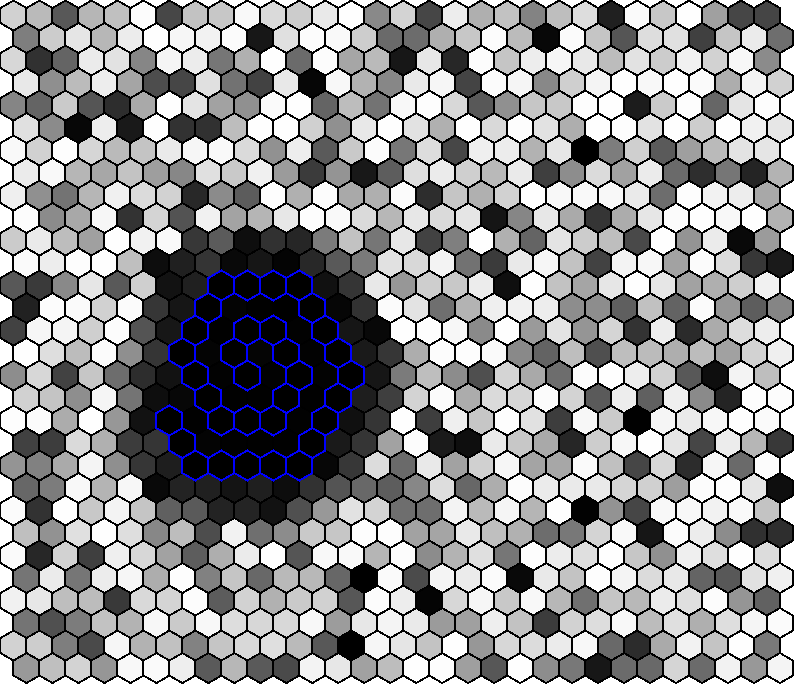
\includegraphics[width=0.25\textwidth]{./images/envH.png}}
  \subfigure[Search Space Estimation after Human Search and Robot Search]{
    \label{fig:envHR:b} %% label for second subfigure 
    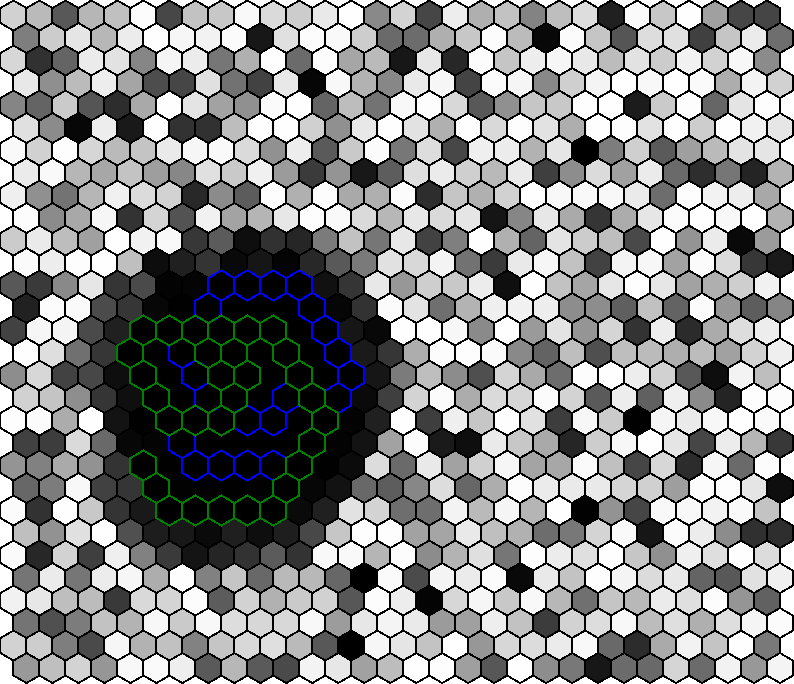
\includegraphics[width=0.25\textwidth]{./images/envHR.png}}
  \subfigure[Problem Size and Search Efficiency as Planning Length increases]{
    \label{fig:pathPlanningIncrease} %% label for second subfigure 
    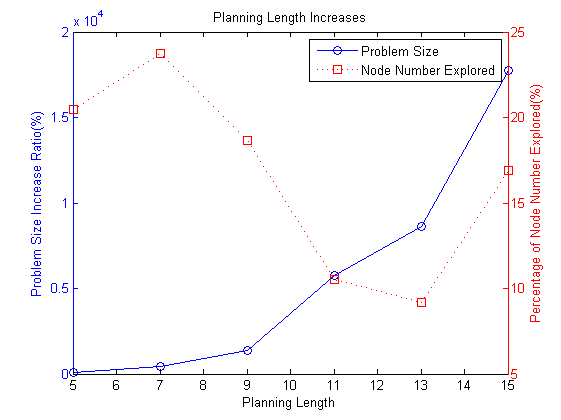
\includegraphics[width=0.32\textwidth]{./images/pathPlanningIncrease.png}}  
  \caption{} 
  \label{fig:envHR} %% label for entire figure 
\end{figure}

Fig.\ref{fig:envHR} shows how the agent search changes the team estimation on the search space. Particularly, in Fig.\ref{fig:envHR:b}, a robot explores the search space after a human search in the wingman constrain to maximize the uncertainty reduction on the team estimation model of the search space. Intuitively, when the planning length increases, the size of the search problem will grow significantly, as shown in Fig.\ref{fig:pathPlanningIncrease}. While the ratio of nodes explored falling leads to better efficiency in larger size of problems.

\subsection{Performance and Efficiency}

There are usually three types of environments to work in, which are ``Uniform Environment", ``Random Environment" and ``Multi-Modal Environment", as in Fig.\ref{fig:diffEnv}.  

\begin{figure}[H] 
  \centering 
  \subfigure[Uniform environment]{ 
    \label{fig:diffEnv:a} %% label for first subfigure 
    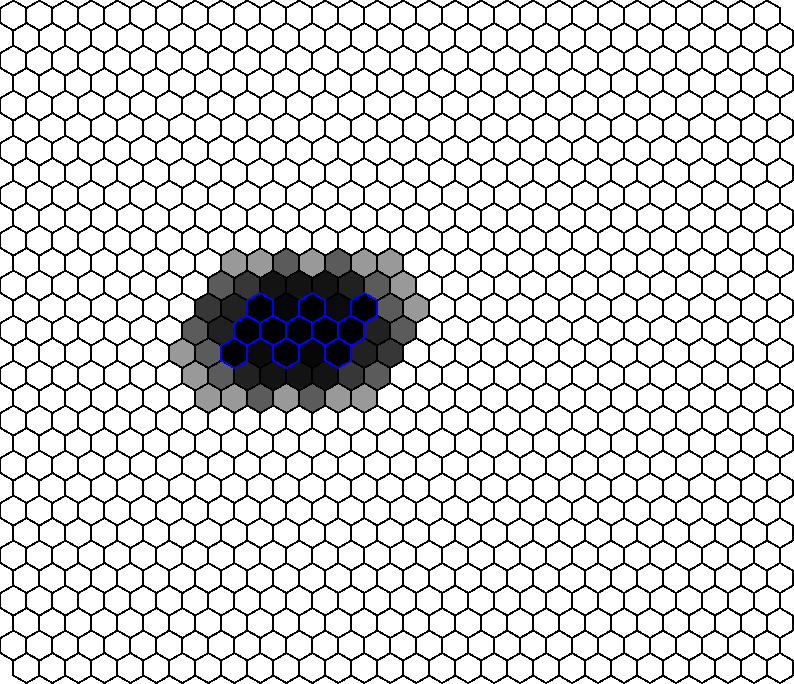
\includegraphics[width=0.3\textwidth]{./images/UniEnv.png}} 
  \subfigure[Random environment]{ 
    \label{fig:diffEnv:b} %% label for second subfigure 
    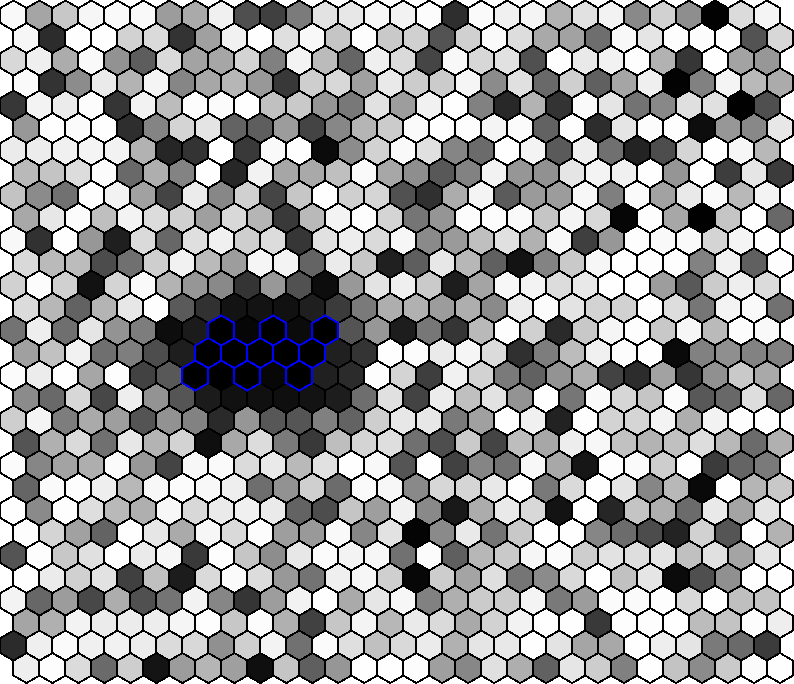
\includegraphics[width=0.3\textwidth]{./images/RndEnv.png}}
  \subfigure[Multi-Modal environment]{ 
    \label{fig:diffEnv:c} %% label for second subfigure 
    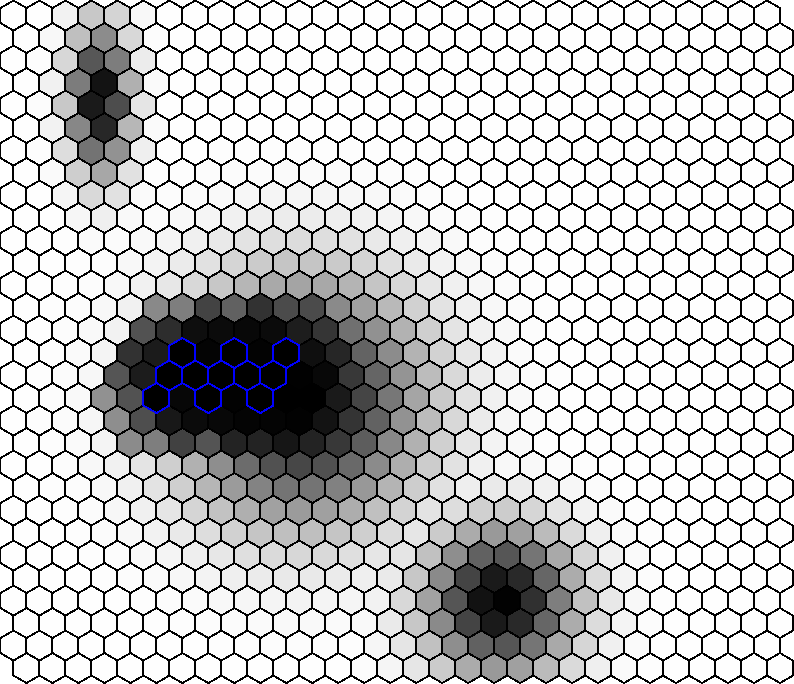
\includegraphics[width=0.3\textwidth]{./images/MMEnv.png}}  
  \subfigure[Performance and efficiency in uniform environment]{ 
    \label{fig:diffEnv:a1} %% label for first subfigure 
    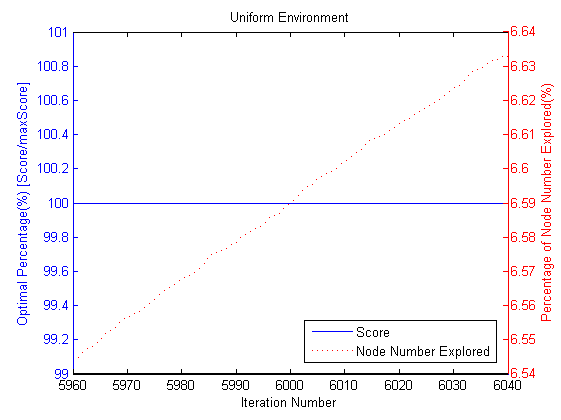
\includegraphics[width=0.3\textwidth]{./images/PM_EnvUni.png}}  
  \subfigure[Performance and efficiency in random environment]{ 
    \label{fig:diffEnv:a2} %% label for second subfigure 
    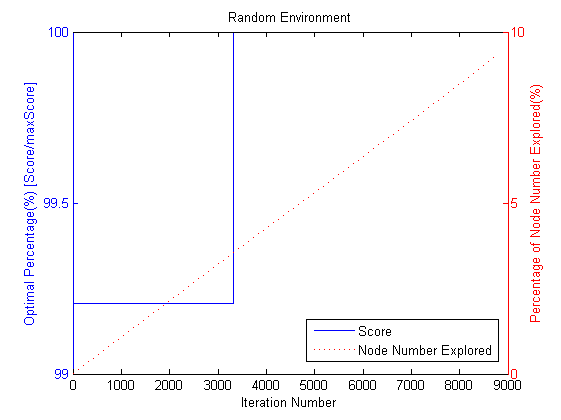
\includegraphics[width=0.3\textwidth]{./images/PM_EnvRnd.png}}
  \subfigure[Performance and efficiency in multi-modal environment]{ 
    \label{fig:diffEnv:a3} %% label for second subfigure 
    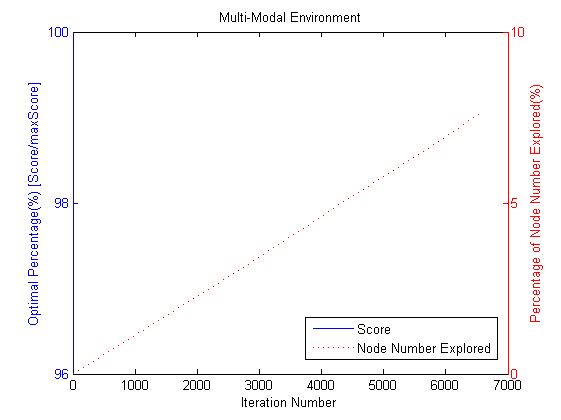
\includegraphics[width=0.3\textwidth]{./images/PM_EnvMM.png}}     
  \caption{} 
  \label{fig:diffEnv} %% label for entire figure 
\end{figure}

Usually ``tree-expanding search with recursive backtracking" works very well in Uniform and Multi-Model Environments, because the estimation on the $ est_{max}(R^{max}_{future}(v)) $ is consistent with the true gradient. In Random Environment, it takes some time to move into optimal solution due to the stochastic pattern of reward distribution. So the other tests are all taken in Random Environment. In all three types of environments, the proposed algorithm explored very small portions of the entire solution spaces, as in Fig.\ref{fig:diffEnv}.

Another factor leads to performance diversity is the pattern of human path, which constrains the solution space in a timed pattern. In Fig.\ref{fig:diffHMP}, five common patterns in search tasks are selected, which are ``Line", ``Spiral", ``Lawn Mower", ``Arc" and "Loitering". In order to compare, they are formed in same planning length, which is 11 in this example. 

\begin{figure}[H] 
  \centering 
  \subfigure[Human path - Line]{ 
    \label{fig:HMP_Line} %% label for first subfigure 
    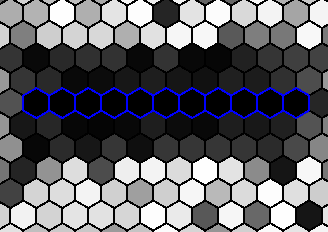
\includegraphics[width=0.2\textwidth]{./images/HMP_Line_Small.png}} 
  \subfigure[Human path - Spiral]{ 
    \label{fig:HMP_Sipral} %% label for second subfigure 
    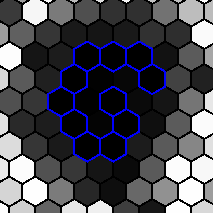
\includegraphics[width=0.14\textwidth]{./images/HMP_Spiral_Small.png}}
  \subfigure[Human path - Lawn Mower]{ 
    \label{fig:HMP_LawnMower} %% label for second subfigure 
    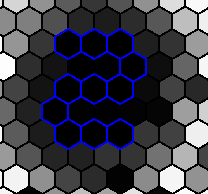
\includegraphics[width=0.14\textwidth]{./images/HMP_LawnMower_Small.png}}  
  \subfigure[Human path - Arc]{ 
    \label{fig:HMP_Arc} %% label for first subfigure 
    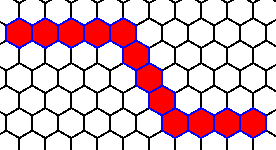
\includegraphics[width=0.2\textwidth]{./images/HMP_Arc_Small.png}} 
  \subfigure[Human path - Loitering]{ 
    \label{fig:HMP_Loitering} %% label for second subfigure 
    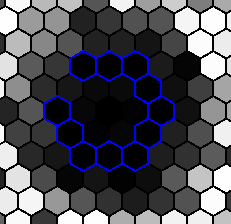
\includegraphics[width=0.14\textwidth]{./images/HMP_Loitering_Small.png}}                
  \caption{Different patterns of human path.} 
  \label{fig:diffHMP} %% label for entire figure 
\end{figure}

In Fig.\ref{fig:ProbSizeIndiffHMP}, it is noticeable that in identical planning length, ``Spiral" and ``Lawn Mower" patterns generates much bigger solution spaces than ``Line" and ``Arc", and ``Loitering" is in between. It shows that the curvature of a human path has a strong influence on the size of solution space. The more overlap between the flank support regions at two neighboring time steps, the higher connectivities between the nodes in two neighboring partites are. As a result, the size of problems grows as the connectivities increase. 

\begin{figure}[H] 
  \centering 
  \subfigure[Sizes of solution spaces in different patterns of human paths]{ 
    \label{fig:ProbSizeIndiffHMP} %% label for first subfigure 
    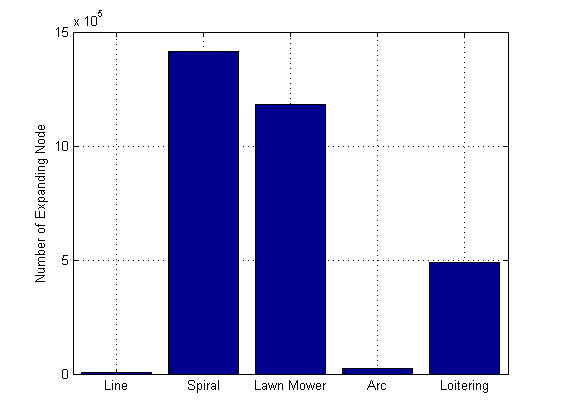
\includegraphics[width=0.45\textwidth]{./images/ProbSizeInDiffHMP.png}} 
  \subfigure[Exploration ratios In different patterns of human paths]{ 
    \label{fig:ExoRatioInDiffHMP} %% label for second subfigure 
    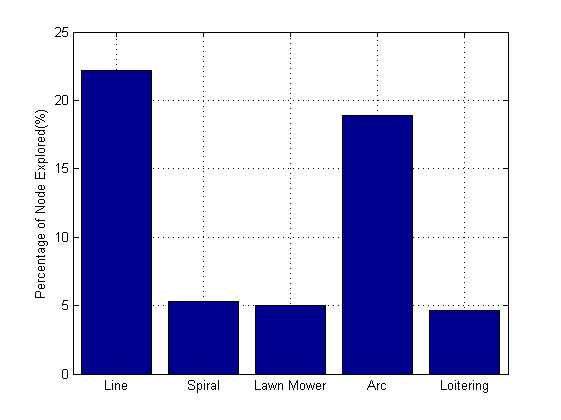
\includegraphics[width=0.45\textwidth]{./images/ExpRatioInDiffHMP.png}}
  \subfigure[Percentages of optimal at first iteration in different patterns of human paths]{ 
    \label{fig:InitOptInDiffHMP} %% label for second subfigure 
    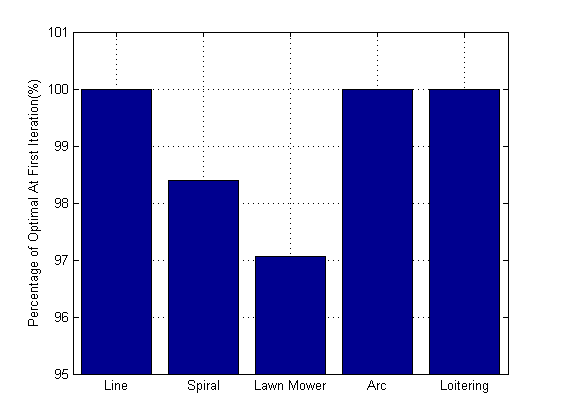
\includegraphics[width=0.45\textwidth]{./images/InitOptInDiffHMP.png}}                 
  \caption{Performances in different patterns of human paths} 
  \label{fig:PMdiffHP} %% label for entire figure 
\end{figure}

With smaller solution spaces, the proposed algorithm has lower efficiencies in finding the optimal in the cases of ``Line" and ``Arc" , as in Fig.\ref{fig:ExoRatioInDiffHMP}. However, due to less coverage overlap, the proposed algorithm has higher percentages of optimality at first iteration from backtracking. 

\subsection{Parameters and Discussion}

\subsubsection{Flank Support Range}

Working with an observation range of each team agent, the flank support range can be considered as a parameter defining the collaborative factor between the human and the robot wingman. Decreasing the support range might enhance peer-to-peer communication and guarantee instant response to others when needed, while increasing the range is likely to bring higher information gathering capacity.

\begin{figure}[H] 
  \centering 
  \subfigure[Sizes of solution spaces in different patterns of human paths]{ 
    \label{fig:ProbSizeIndiffWR} %% label for first subfigure 
    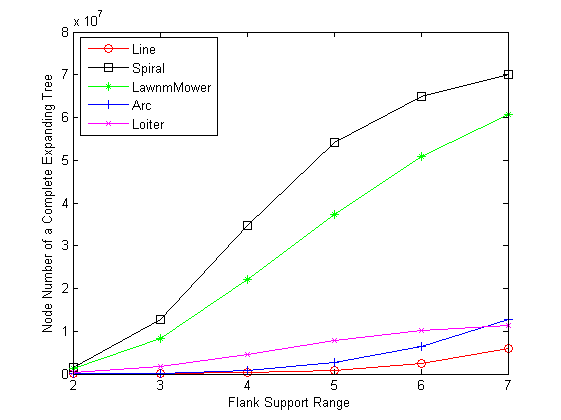
\includegraphics[width=0.45\textwidth]{./images/ProbSizeInDiffWR.png}} 
  \subfigure[Optimal scores in different patterns of human paths]{ 
      \label{fig:OptScoreIndiffWR} %% label for first subfigure 
      \includegraphics[width=0.45\textwidth]{./images/OptScoreIndiffWR.png}}   
  \subfigure[Ratios of exploration in different patterns of human paths]{ 
    \label{fig:ExoRatioInDiffWR} %% label for second subfigure 
    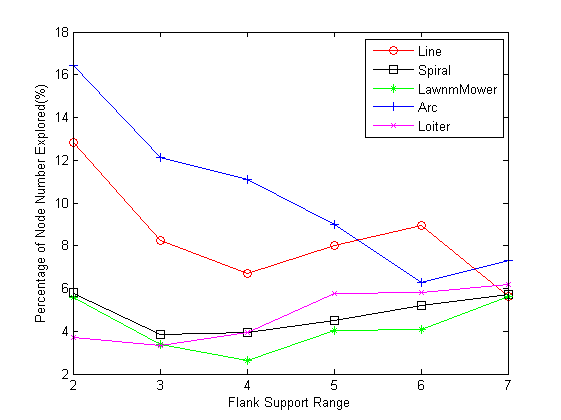
\includegraphics[width=0.45\textwidth]{./images/ExpRatioInDiffWR.png}}
  \subfigure[Percentages of optimal at first iteration in different patterns of human paths]{ 
    \label{fig:InitOptInDiffWR} %% label for second subfigure 
    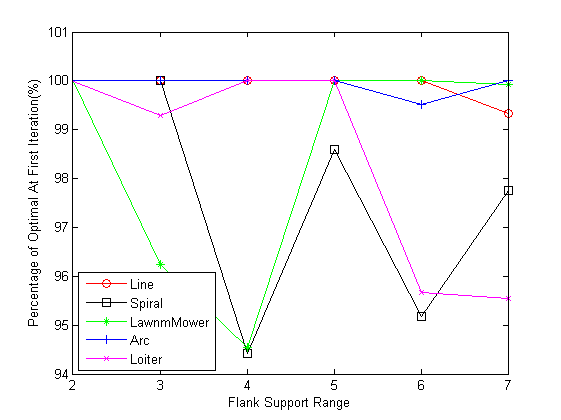
\includegraphics[width=0.45\textwidth]{./images/InitOptInDiffWR.png}} 
  \subfigure[Percentages of total iterations when reaching optimal in different patterns of human paths]{ 
    \label{fig:OptHitInDiffWR} %% label for second subfigure 
    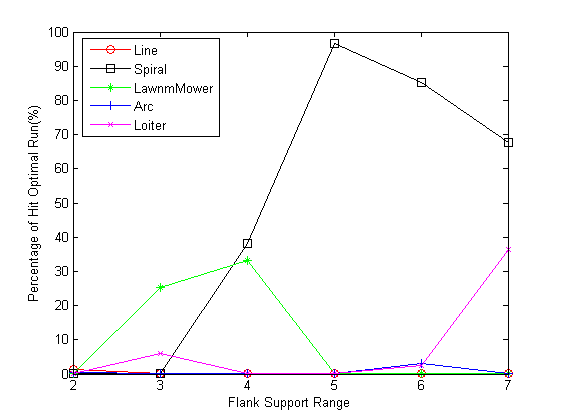
\includegraphics[width=0.45\textwidth]{./images/OptHitInDiffWR.png}}                       
  \caption{When the flank support range is increased} 
  \label{fig:PMdiffWR2} %% label for entire figure 
\end{figure}

In Fig.\ref{fig:ProbSizeIndiffWR}, it shows that increasing the flank support range leads to the increase on the size of solution space, especially in the cases of ``Spiral" and ``Lawn Mower". When the flank support range is increased to some level, the increase of the rewards falls down, as in Fig.\ref{fig:OptScoreIndiffWR}. Consistently, when the sizes of the solution spaces increases with the flank support range, the efficiencies of the proposed algorithms become higher in Fig.\ref{fig:ExoRatioInDiffWR}. Due to bigger sizes of solution spaces and higher overlaps of coverages, Fig.\ref{fig:InitOptInDiffWR} show that the algorithm has less chance to reach the optimal in the first iteration in the cases of ``Spiral" and ``Lawn Mower", though the percentages of optimality are high enough. Especially it takes longer time to reach the optimal in the cases of ``Spiral" and ``Lawn Mower". The growths of the sizes of solution spaces also make the algorithm harder to find the optimal in the cases of ``Spiral" and ``Lawn Mower". But Fig.\ref{fig:OptHitInDiffWR} shows that they start to fall when the flank support range reaches some level, when the optimal score is close to saturation.


\subsubsection{Observation Model}

How the observation model of the agents are like also has influence on the performance of the algorithms. Two factors are looked at in this paper, which are the human observation range and the robot observation range.

\paragraph{Human Observation Range}

When increasing the human observation range, the human observation will take more uncertainty away from the environment model. Fig.\ref{fig:ExoRatioInDiffHR} illustrates that . There is very little influence on the percentages of optimality at the first iteration in all cases, as in Fig.\ref{fig:InitOptInDiffHR}. It is only noticeable that in the case of ``Lawn Mower", which is good for cleaning up uncertainty of a region, the efficiency of the algorithm has been influenced, in Fig.\ref{fig:OptHitInDiffHR}. But when the observation range number increased to some level, means that the uncertainty of the region can be well cleaned up, the performance of the algorithm becomes consistent.

\begin{figure}[H] 
  \centering 
  \subfigure[Ratios of exploration in different patterns of human paths]{ 
    \label{fig:ExoRatioInDiffHR} %% label for second subfigure 
    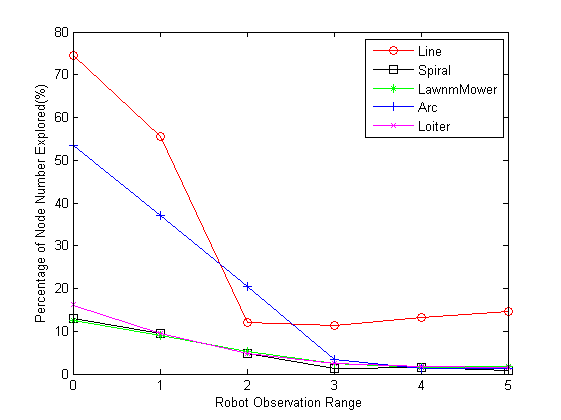
\includegraphics[width=0.45\textwidth]{./images/ExpRatioInDiffHR.png}}
  \subfigure[Percentages of optimal at first iteration in different patterns of human paths]{ 
    \label{fig:InitOptInDiffHR} %% label for second subfigure 
    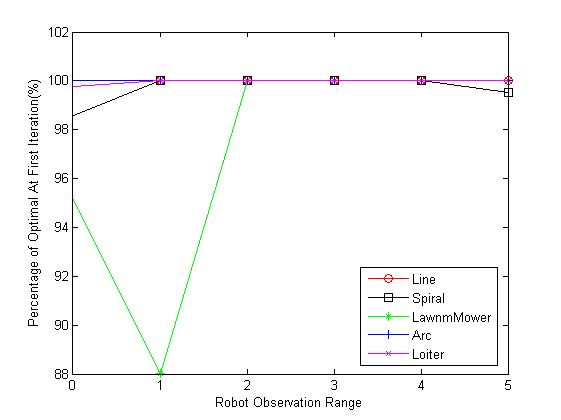
\includegraphics[width=0.45\textwidth]{./images/InitOptInDiffHR.png}} 
  \subfigure[Percentages of total iterations when reaching optimal in different patterns of human paths]{ 
    \label{fig:OptHitInDiffHR} %% label for second subfigure 
    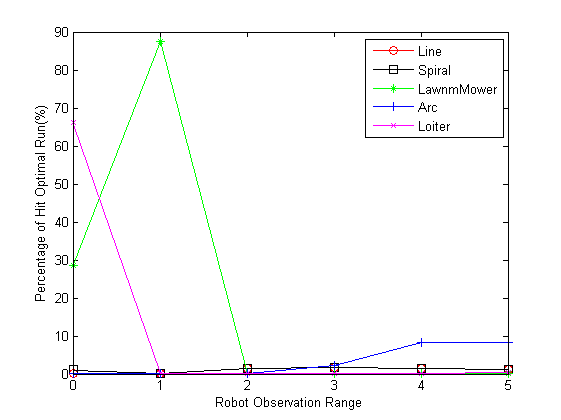
\includegraphics[width=0.45\textwidth]{./images/OptHitInDiffHR.png}}                       
  \caption{When the human observation range is increased} 
  \label{fig:PMdiffHR} %% label for entire figure 
\end{figure}

\paragraph{Robot Observation Range}

When increasing the robot observation range, there will be bigger overlap on the observation coverages between two neighboring steps. Opposite to the growths of the sizes of solution spaces, the proposed algorithm shows less efficiently in the cases of ``Spiral" and ``Arc" in Fig.\ref{fig:ExoRatioInDiffRR}, which have less overlap between observation coverages between two neighboring steps when the observation range is relatively small. However, the algorithm can actually reach the optimal very quickly in these two cases as in Fig.\ref{fig:InitOptInDiffRR} and Fig.\ref{fig:OptHitInDiffRR}. It needs relatively a longer time to converge to the correct estimation from backtracking. Also in the case of "Lawn Mower", the proposed algorithm shows a  

\begin{figure}[H]
  \centering 
  \subfigure[Ratios of exploration in different patterns of human paths]{ 
    \label{fig:ExoRatioInDiffRR} %% label for second subfigure 
    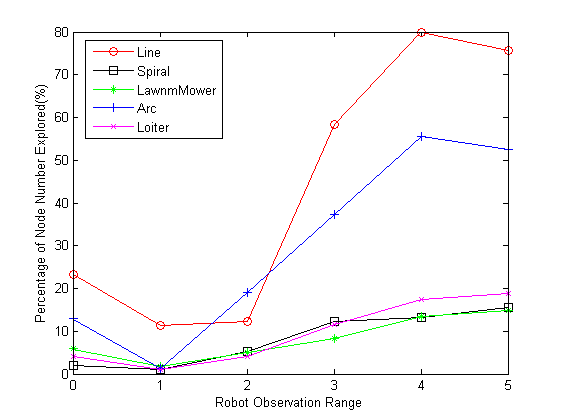
\includegraphics[width=0.45\textwidth]{./images/ExpRatioInDiffRR.png}}
  \subfigure[Percentages of optimal at first iteration in different patterns of human paths]{ 
    \label{fig:InitOptInDiffRR} %% label for second subfigure 
    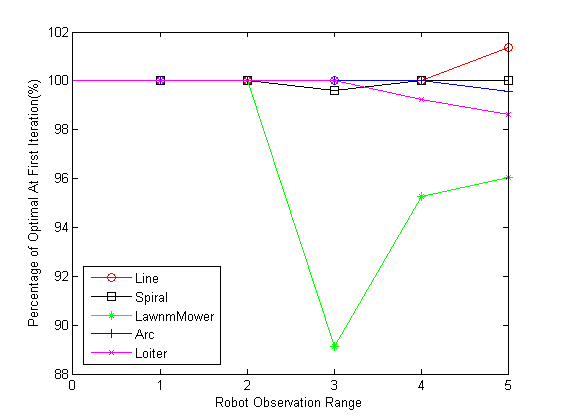
\includegraphics[width=0.45\textwidth]{./images/InitOptInDiffRR.png}} 
  \subfigure[Percentages of total iterations when reaching optimal in different patterns of human paths]{ 
    \label{fig:OptHitInDiffRR} %% label for second subfigure 
    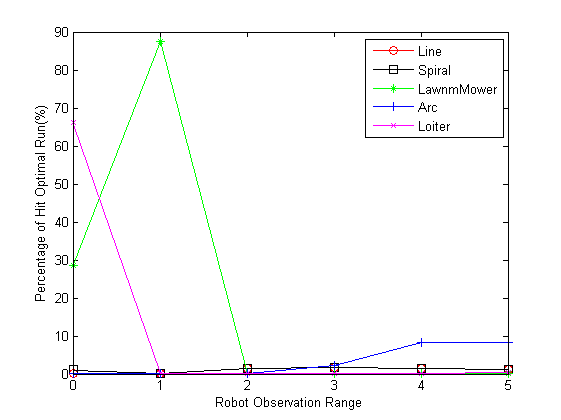
\includegraphics[width=0.45\textwidth]{./images/OptHitInDiffHR.png}}                       
  \caption{When the robot observation range is increased} 
  \label{fig:PMdiffRR} %% label for entire figure 
\end{figure}


\subsubsection{Obstacle}
The existence of obstacles often breaks the connectivity between cells. In the way we discretize the search space, an obstacle will make some vertices in the graph inaccessible, and as a result we will remove those inaccessible vertices from multi-partite graph, which might generate some vertices which has zero in-degree or zero out-degree. However, the pruning process will remove those vertices. So here obstacles only bring the reduction of vertices which decreases the size of search graph.

\section{Summary}

The information maximization path planning of a robot wingman has been formed as a generic path-dependent optimization problem. The algorithm of tree-expanding with recursive backtracking is proposed and proved to be efficient and convergent to optimal in different patterns of human paths and environments. It always shows optimal or near-optimal solution at the first iteration, especially when the human path is less curvy. It can also keep on iterating to refine the solution and provides performance guarantee. It also shows significant increase on search efficiency when the size of the problem becomes large.  


\bibliographystyle{apalike}
\bibliography{reference}

\end{document}
